\documentclass[UKenglish]{ifimaster}
\usepackage[latin1]{inputenc}
\usepackage[T1]{url}
\usepackage{babel,textcomp,uiosloforside,varioref,graphicx}
\usepackage{tikz}
\urlstyle{sf}

\title{CloudML}
\subtitle{A DSL for model- and web-based realisation of applications in the cloud}
\author{Eirik Brandtz�g}
\date{Spring 2012}

\begin{document}
\uiosloforside{}

\frontmatter{}
\maketitle{}

\chapter*{Abstract}

\tableofcontents{}
\listoffigures{}
\listoftables{}

\chapter*{Preface}

\mainmatter{}
\part{Introduction}
\chapter{Terminology table}

\begin{table}
    \caption{Terminologies}
    \begin{tabular}{ | l | p{10cm} | }
      \hline
      \textbf{Word} & \textbf{Meaning} \\
      \hline
      Instance & Virtual machine instance. \\ \hline
      Resource & Set of services that a cloud provider support.
      Can be a instance, storage capacity, geographical location, SSO. Some are physical for the user, others are automatical. \\ \hline
      Stack & Set of resources. \\ \hline
      Provider & Company that makes a business of selling cloud solutions. Such as Amazon (AWS), Rackspace, Azure and Linode. \\ \hline
      Profile & Part of CloudML used to represent Resources for other providers. \\ \hline
      CloudFormation & Amazon AWS CloudFormation \\ \hline
    \end{tabular}
\end{table}

\chapter{Problem}
There are many cloud providers on the global market today. These providers support many layers of cloud, 
such as PaaS (Platform as a Service) and IaaS (Infrastructure as a Service). 
This vast amount of providers and new technologies and services can be overwhelming for many companies and small and medium businesses. 
There are no practical introductions to possibilities and limitations to cloud computing, or the differences between different providers and services. 
Each provider has some kind of management console, usually in form of a web interface and API. 
But model driven approaches are inadequate in many of these environments. 
UML diagrams such as deployment diagram and component diagram are used in legacy systems to describe system architectures, 
but this advantage has yet to hit the mainstream of cloud computing management. 
It is also difficult to have co-operational interaction on a business level without using the advantage of graphical models.
The knowledge needed to handle one provider might differ to another, so a multicloud approach might be very resource-heavy on competence in companies. 
The types of deployment resources are different between the providers, even how to gain access to and handle running instances might be very different. 
Some larger cloud management application developers are not even providers themselves, but offer tooling for private cloud solutions.
Some of these providers have implemented different types of web based applications that let end users manage their cloud instances. 
The main problem with this is that there are no standards defining a cloud instance or links between instances and other services a provider offer.
If a provider does not offer any management interface and want to implement this as a new feature for customers, 
a standard format to set the foundation would help them achieve a better product for their end users.
These are some of the problems with cloud hosting today, and that CloudML will be designed to solve.

\chapter{Analysis}
\section{Amazon AWS CloudFormation}
\url{http://aws.amazon.com}

This is a service provided by Amazon from their popular Amazon Web Services. 
It give users the ability to create template files in form of JSON, which they can load into AWS to create stacks of resources. 
This makes it easier for users to duplicate a setup many times, and as the templates support parameters this process 
can be as dynamic as the user design it to be. This is a model in form or lexical syntax, both the template itself and the resources that can be used.
For a company that is fresh in the world of cloud computing this service could be considered too advance. 
This is mainly meant for users that want to replicate a certain stack, with the ability to provide custom parameters. 
Once a stack is deployed it is only maintainable through the AWS Console, and not through template files. 
The format that Amazon uses for the templates is a very good format, the syntax is in form of JSON which is very readable and easy to use, 
but the structure and semantics of the template itself is not used by any other providers or cloud management tooling, 
so it can not be considered a multicloud solution. Even though JSON is a readable format, does not make it viable as a presentation medium on a business level.

\section{CA Applogic}
\url{http://www.3tera.com/AppLogic/}

Applogic from CA is a proprietary model based web application for management of private clouds. 
This interface let users configure their deployments through a diagram with familiarities to component diagrams with interfaces and assembly connectors. 
This is one of the solutions that use and benefit from a model based approach. They let users configure a selection of third party applications, 
such as Apache and MySQL, as well as network security, instances and monitoring. 
What CA has created is both an easy way into the cloud and it utilizes the advantages of model realizations. 
Their solution will also prove beneficial when conducting business level consulting. 
They also support a version of ADL (Architecture Deployement Language), a good step on its way to standardization. 
But this solution is only made for private clouds running their own controller, this can prove troublesome for migration, both in to and out of the infrastructure.

\section{libcloud and jclouds}
\url{http://libcloud.apache.org/}
\url{http://www.jclouds.org/}

Libcloud is a API that aims to support the largest cloud providers through a common API. 
The classes are based around "Drivers" that extends from a common ontology, then provider-specific attributes and logic is added to the implementation.
jclouds is very similar to libcloud but the API code base is written in Java and Clojure. 
This library also have "drivers" for different providers, but they also support some PaaS solutions such as Google App Engine.
APIs can be considered modelling approaches based on the fact they have a topology and hierarchical structure, 
but it is not a distinct modelling. A modelling language could overlay the code and help providing a clear overview, 
but the language directly would not provide a good overview of deployment. 
And links between resources can be hard to see, as the API lacks correlation between resources and method calls. 
Libcloud have solved the multicloud problem in a very detailed manner, but the complexity is therefore even larger. 
The API is also Python-only and could therefor be considered to have high tool-chain dependency.

\section{OPA}
\url{http://opalang.org/}

OPA is a cloud language aimed at easing development of modern web applications. It is a new language, 
with its own syntax, which is aimed directly at the web. The language will build into executable files that will handle load balancing and scalability, 
this is to to make this a part of the language and compilation.
OPA is a new language, so it might be difficult to migrate legacy systems into this lanugage. 
There are no deployment configurations, as this is built into the language. The compiler will generate an executable that coWeb-based vs native application

The public cloud is located on the world wide web, and most of the managing, monitoring, 
payment and other administrative tasks can be done through web interfaces or APIs. 
Web applications are becoming more popular by the day, with HTML5, EcmaScript 5 and CSS3. 
The user experience in web applications today can in many cases match native applications, with additional benefits such as availability and ease of use.
A web-based interface would prove beneficial for quickly displaying the simple core functionality of the language. 
In this era of cloud computing and cloud technologies a user should not need to abandon his or hers browser to explore the functionality of CloudML.
Cloud providers are most likely to give customers access to customize their cloud services through web-based interfaces, 
and if customers are to take advantage of CloudML, the language should be graphically integrated into existing tool chains. 
Providers would probably find it pleasing if a example GUI wauld be run on most cloud providers instances, 
and so it can also benefit from some cloud based load balancers, even though this is part of the language. 
The conclusion about OPA is that it is not a language meant for configuration, and could not easily benefit from a model based approach, 
and it does not intentionally solve multicloud.

\section{Whirr}
\url{http://whirr.apache.org/}

This is a binary and code-based application for creating and starting short-lived clusters for hadoop instances.
It support multiple cloud providers. It has a layout for configuration but it is mainly property-based, and aimed at making clusters. 

\section{Deltacloud}
\url{http://incubator.apache.org/deltacloud/}

Deltacloud has a similar procedure as jclouds and libcloud, but with a REST API. 
So they also work on the term "driver", but instead of having a library to a programming language the users are presented with an API they can call, 
on Deltacloud servers. This means users can write in any language they may choose. 
As well as having similar problems as other APIs this approach means that every call has to go through their servers, 
similar to a proxy. This can work with the benefits that many middleware software have, such as cahing, queues, 
redundancy and transformations, but it also has the disadvantages such as single point of failure and version inconsistencies.

\section{Table}
\begin{table}
    \caption{Analysis}
    \begin{tabular}{ | p{2cm} | p{2cm} | p{2.5cm} | p{2cm} | p{2cm} | p{2cm} |}
      \hline
      \textbf{Solution} & \textbf{Easy to start with} & \textbf{Business level viable} & \textbf{Model driven} & \textbf{Multicloud} & \textbf{Standard} \\
      \hline
     Amazon CloudFormation & No & No & No & No & No \\ \hline
     CA Applogic & Yes & Yes & Yes & No & No \\ \hline
     Libcloud & No  & No & No & Yes & No \\ \hline
     jclouds & No & No & No & Yes & No \\ \hline
     OPA & Yes & No & No & No & No \\ \hline
     Whirr & No & No & No & Yes & No \\ \hline
     Deltacloud & No & No & No & Yes & No \\ \hline
    \end{tabular}
\end{table}

\chapter{Requirements}
\section{Table}
\section{Table}
\begin{table}
    \caption{Requirements}
    \begin{tabular}{ | l | p{7cm} | l | }
      \hline
      \textbf{Requirement} & \textbf{Short description} & \textbf{Importance} \\ \hline
      Lexical model & Language should be based on a lexical model. & 3 \\ \hline
      Graphical model & Lexical model should be represented in diagrams. & 2 \\ \hline
      Multicloud & The language should work against more than one provider. & 2 \\ \hline
      Adaptable (?) & Providers should be able to express what they offer according to the CloudML vocabulary to support automation. & 3 \\ \hline
      Executable & The language will be accompanied by an execution engine able to process it and perform static analysis on a given CloudML file. & x \\ \hline
      API & The language should be easy to use through an API. & x \\ \hline
      Versoning (VCS) & The lexical language should be easy to maintain in a VCS such as Git, Mercurial or SVN. & x \\ \hline
    \end{tabular}
\end{table}

\section{Model}
\subsection{Lexical}
When approaching a global audience consisting of both academics and professional providers it is important to create a solid foundation, 
which also should be concrete and easy to both use and implement.
The best approach would be to support both graphical and lexical models, 
but a graphical annotation would not suffice when promising simplicity and ease in implementation. 
Graphical model could also be much more complex to design, while a lexical model can define a concrete model on a lower level.
Since the language will be a simple way to template configuration, a well known data markup language would be sufficient for the core syntax, such as JSON or XML.

\subsection{Graphical}
A graphical representation of CloudML is important as users should recognize the annotation and feel comfortable with it. 
Strict, concrete and simple lexical syntax based on a data structured language should work as core for a graphical annotation. 
An UML profile could be used over component diagrams, but any notation should be sufficient. 
One fundamental advantage about graphical models are helpfulness in affiliations with commercial and business accountables.

\section{Multicloud}
One of the biggest problems with the cloud today is the vast amount of different providers. 
There are usually few reasons for large commercial delegates to have support for contestants. 
Some smaller businesses could on the other hand benefit greatly of a standard and union between providers.
The effort needed to construct a reliable, stable and scaling computer park or datacenter will withhold commitment to affiliations. 
Cloud computing users are concerned with the ability to easily swap between different providers, this because of security, 
independence and flexibility. CloudML and its engine need to apply to several providers with different set of systems, 
features, APIs, payment methods and services. This requirement anticipate support for at least two different providers such as Amazon AWS and Rackspace.

\section{Executable}
The language must be dependant of an underlying engine, this is because creating stacks can be in form of a process, 
and the language should not be an impediment for deployment flows. The engine will not be a part of the PIM version of CloudML, 
but the language must reinforce this reasoning.

\section{API}
The engine underlying CloudML should be easily accessible on a state of the art basis. 
This is most correctly achieved by implementing an REST based API, which can process CloudML template files correctly. 

\section{Versoning}
The file format should be in such form it can be stored a VCS system such as Git, Subversion or Mercurial. 
This is important for end users to be able to maintain templates that defines the stacks they have built, for future reuse.

\section{Granularity}
Cloud computing is often defined into different categories, such as IaaS (Infrastructure as a Service), 
PaaS (Platform as a Service) and SaaS (Software as a Service), although for CloudML it needs to narrow it down or rather redefine our point of view.
The concepts around the language are not defined by what levels of a vendor management responsibilities it should support, 
but rather more concretely what parts of a system stack that can be configured.

\begin{figure}
  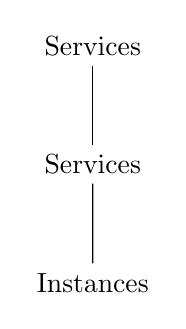
\begin{tikzpicture}
    \node [rectangle] {Services} 
    child {node [rectangle] {Services}
    child {node [rectangle] {Instances}}};
  \end{tikzpicture}
  \caption{Cloud layers}
\end{figure}

The figure above, Figure 1, show the different layers that CloudML can and should support. 
The top most level is services that a provider might support, such as CDN, geo-based serving, monitoring and load balancing. 
All in all services that are external from customers actual application, but that can influence or monitor it.
The next level is software, this is for any software that are co-existing with or for the customers application, 
such as databases, application servers, logging services. All in all software that are running on the same instance as the application, 
but that the customer would like to have automatically or semi-automatically configured and reconfigured.
On the bottom there are two levels, both representing instances. In the instance-level CloudML should bind together instances 
such as different virtual machines. This level is tightly connected to the Software-layer as connections between instances 
is very likely to be defined through software, such as databases, web accelerators and application servers.

\chapter{Background}

\part{The project}

\chapter{Planning the project}

\part{Conclusion}

\chapter{Results}

\backmatter{}
\bibliographystyle{plain}
\end{document}
